\subsection{Einrichten der Projektumgebung}
Für die Entwicklung der \ac{pwa} wird die Entwicklungsumgebung \textit{Webstorm} von JetBrains gewählt, da sie die viele Routineaufgaben selbstständig beziehungsweise mit geringem Aufwand ausführt.

Wie für die Entwicklung der meisten modernen Webanwendungen ist die Installation der \textit{Node.js} Laufzeitumgebung notwendig. Mit dem integrierten Paketmanager \textit{npm} lassen sich Bibliotheken leicht zum Projekt hinzufügen.
Um die \textit{Angular} Anwendung automatisiert zu erstellen, ist zuerst die Installation des Angular \acf{cli} erforderlich. Mit dem Konsolenbefehl \texttt{npm install -g @angular/cli} wird npm aufgefordert, die neuste Version der Angular \ac{cli} global auf dem System zu installieren.


Mit dem Befehl \texttt{ng new todoapp} wird die Angular \ac{cli} (in der Konsole als \texttt{ng} abgekürzt) dazu gebracht, ein Angularprojekt inklusive nötiger Dateistrukturen zu erstellen.
\begin{wrapfigure}{r}{0.6\textwidth}
	\vspace{-10pt}
	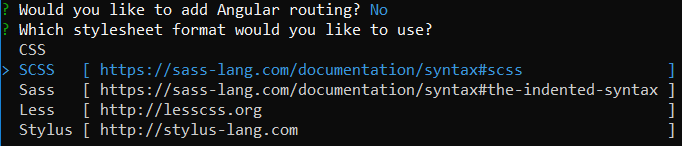
\includegraphics[width=0.58\textwidth]{img/angular_cli_css.PNG}
	\caption{Stylesheetformate beim Erstellen der Angularanwendung}
	\label{fig:stylesheet_formate_cli}
	\vspace{-10pt}
\end{wrapfigure}
Die \ac{cli} bietet dem Nutzer einige Optionen bei der Erstellung an, die jedoch in diesem Projekt nicht zwangsläufig benötigt werden, so kann beispielsweise ein Routing oder Unittesting eingerichtet werden.
Außerdem unterstützt die \ac{cli} verschiedene Stylesheetformate (siehe Abbildung \ref{fig:stylesheet_formate_cli}). Das ist für Entwickler*innen sehr praktisch, wenn sie einen dieser CSS-Dialekte beherrschen. Die Arbeit mit Variablen in Stylesheets bevorzugt wird, werden in diesem Projekt SCSS Dateien verwendet.


\subsection{Umsetzung der Anwendung mit Angular}

Im Folgenden werden die einzelnen Komponenten der \textit{Angular}-Anwendung erläutert. Es wird explizit darauf hingewiesen, dass \textbf{Quellcode-Ausschnitte teilweise stark gekürzt worden sind}, um die Lesbarkeit zu erhöhen.

\subsubsection{Klasse \texttt{TodoItem} zur Datenspeicherung}

Die Komponenten tauschen untereinander Daten aus. Damit diese einer einheitlichen Struktur folgen, wird eine Klasse \texttt{TodoItem} erstellt, die einen Todo-Eintrag repräsentiert. Objekte dieser Klasse können jetzt einfach zwischen Komponenten ausgetauscht und modifiziert werden.

\begin{listing}[h]
	\inputminted{TypeScript}{sourcecode/pwa_todoitem_klasse.js}
	\caption{\texttt{TodoItem}-Klasse zur Datenspeicherung (gekürzt)}
	\label{sourcecode:todoitem_klasse}
\end{listing}

Wie im Ausschnitt \ref{sourcecode:todoitem_klasse} zu sehen, hat ein Todo-Element eine Aufgabenbeschreibung (Zeile 2), zwei boolesche Werte, die speichern, ob das Element als wichtig oder abgeschlossen markiert worden ist (Zeile 4 und 5) und eine eindeutige ID (Zeile 2). Die ID hilft später ein bestimmtes Todo-Element zu modifizieren.

\subsubsection{Erstellund des \texttt{todoService} für die Datenverwaltung}
Alle Todo-Einträge sollen persistent auf dem Gerät gespeichert werden. Dafür wird ein Angular-Service erstellt: der \texttt{todoService}. Er ist für die \acf{crud} Operationen zuständig.

\begin{listing}[h]
	\inputminted{TypeScript}{sourcecode/pwa_todo_service.ts}
	\caption{Klasse \texttt{TodoService} (gekürzt)}
	\label{sourcecode:pwa_todo_service}
\end{listing}

In Ausschnitt \ref{sourcecode:pwa_todo_service} sind die Kernfunktionen des Services abgebildet. Der Service speichert ein Array von \texttt{TodoItem}-Objekten. Wenn der*die Nutzer*in ein Element hinzufügt, erstellt der Service ein neues Datenobjekt und speichert dieses im Array und dem Browserspeicher (Zeilen 16-18). Die Funktionsweise der übrigen \ac{crud}-Operationen ist analog dazu.

Mit \texttt{localStorage} (Zeilen 8-14) kann auf den\textit{ Key-Value-Store} des Browsers zugegriffen werden. Beim Speichern werden die Todo-Elemente als \ac{json}-Objekt im Store abgelegt und analog dazu geladen. Der Key-Value-Store verliert seine Daten beim schließen der Seite nicht und besitzt kein Ablaufdatum, wie ein Cookie \cite{LocalStorage}.

\begin{figure}[h]
	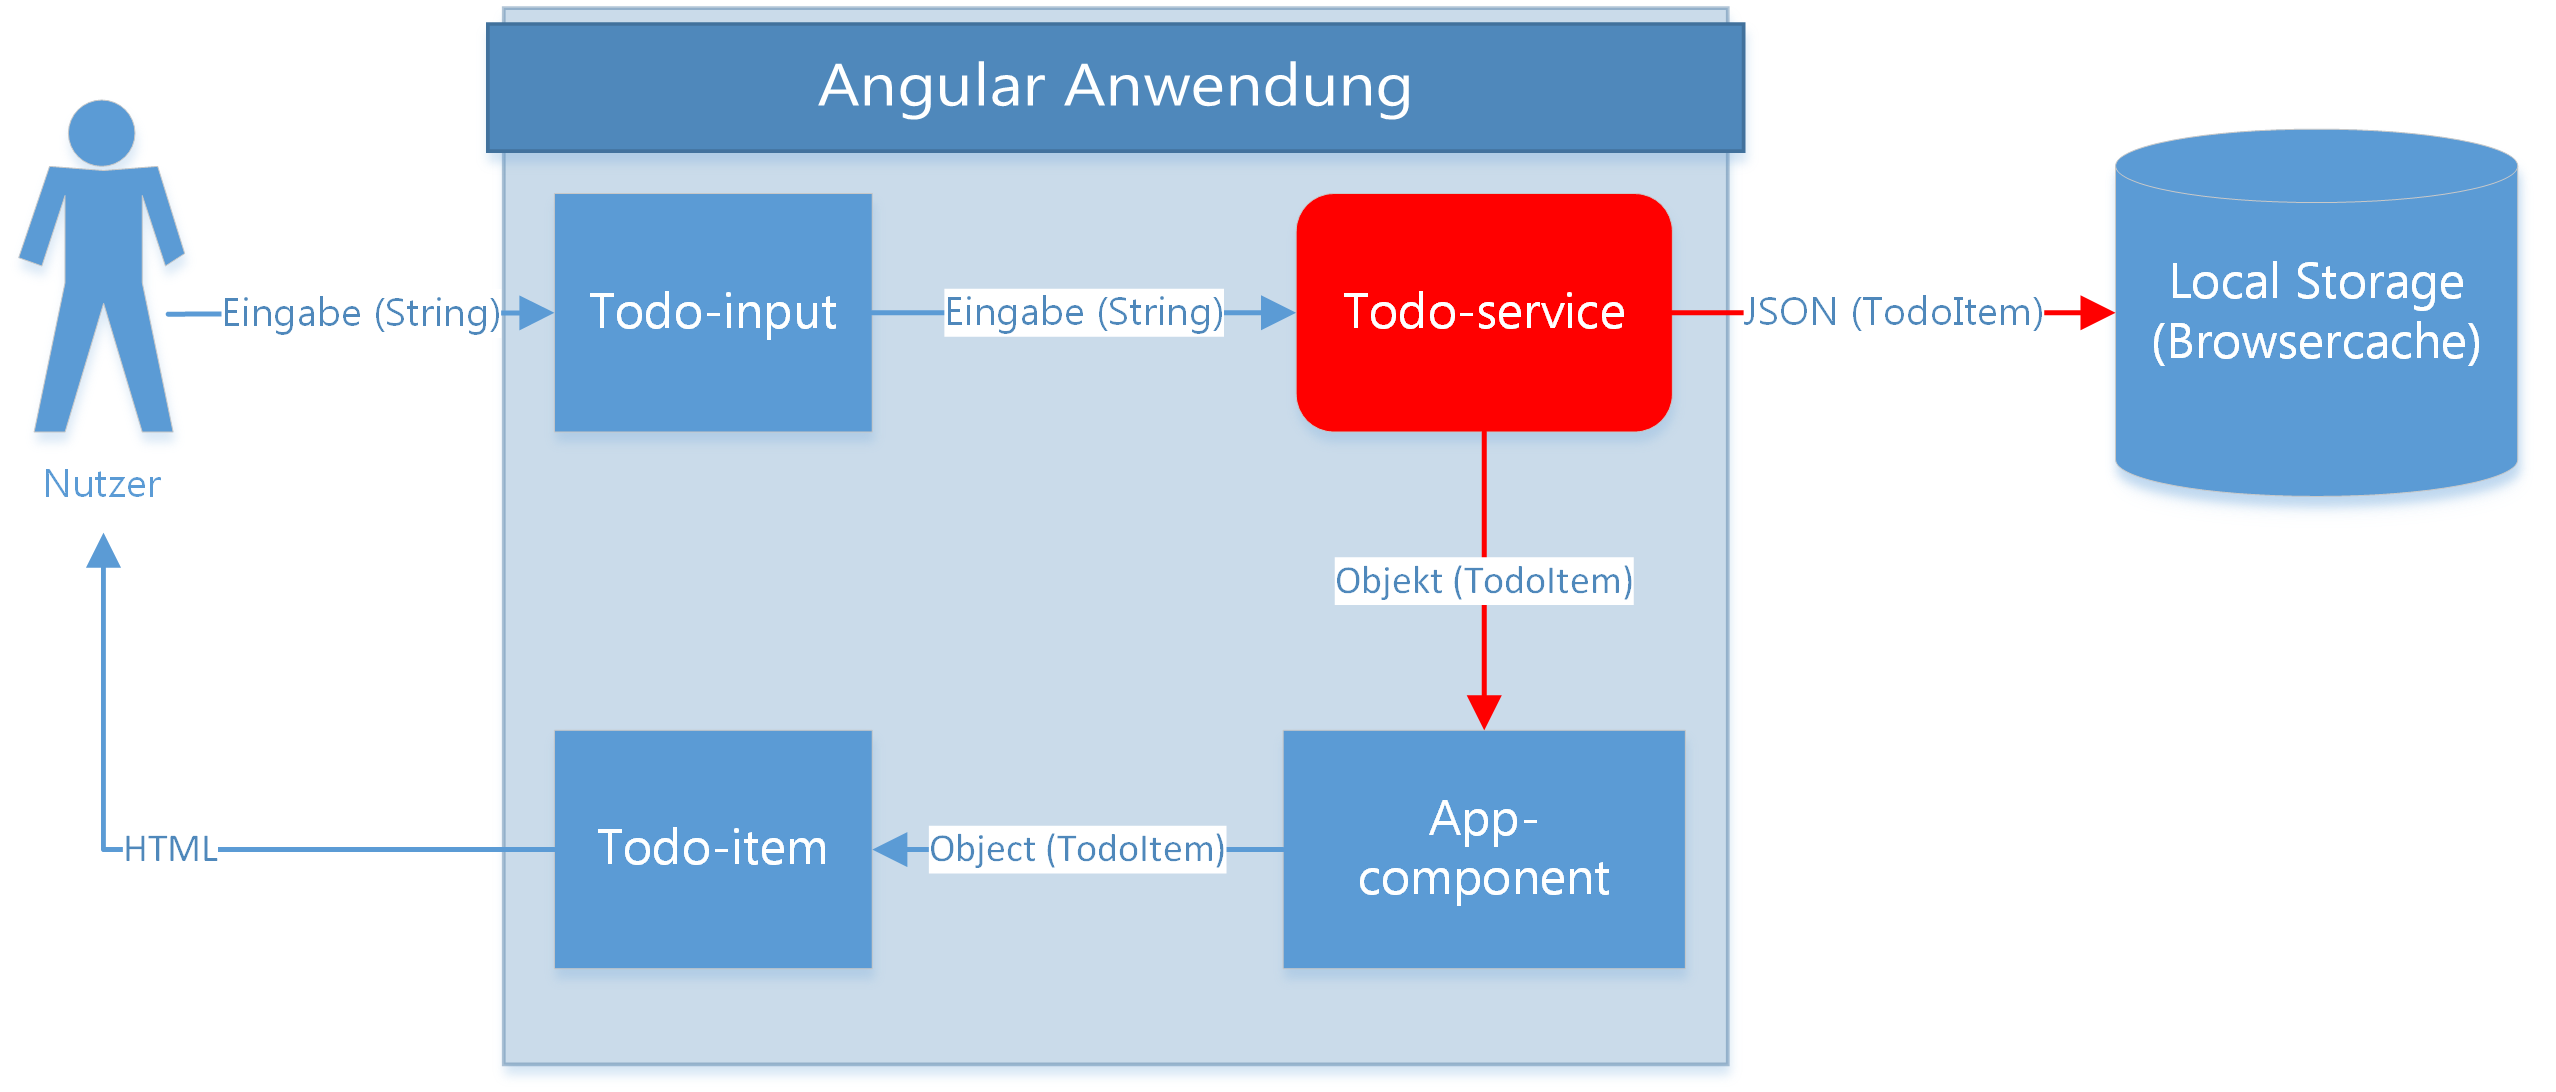
\includegraphics[width=\textwidth]{img/pwa_datenfluss_erstellen.png}
	\centering
	\caption{Datenfluss bei Erstellung eines Todo Eintrages}
	\label{fig:pwa_datenfluss_erstellen}
\end{figure}

Abbildung \ref{fig:pwa_datenfluss_erstellen} zeigt den Datenfluss beim Erstellen eines Todo-Eintrags. Die Todo-Beschreibung wird vom Nutzer*in über ein Eingabefeld an den Service weitergereicht. Dieser erstellt ein entsprechendes Datenobjekt und reicht es der Stammkomponente weiter, worüber schlussendlich HTML-Code erzeugt werden kann. Gleichzeitig speichert er das neue Element im Browserspeicher ab.

\subsubsection{Dateistruktur und Komponenten der Angularanwendung}
Nach dem im Vorangegangenen beschrieben worden ist, wie das Projekt erstellt worden ist, wird im Folgenden detaillierter auf das erstellte \textit{Angular}-Projekt eingegangen. Angular, welches stark komponentenorientiert aufgebaut ist, zeigt sich auch in seiner Dateistruktur stark komponentenbezogen. In Abbildung \ref{fig:pwa_dateistruktur} sind die wichtigsten Dateien in einem Diagramm dargestellt.

\begin{figure}[H]
	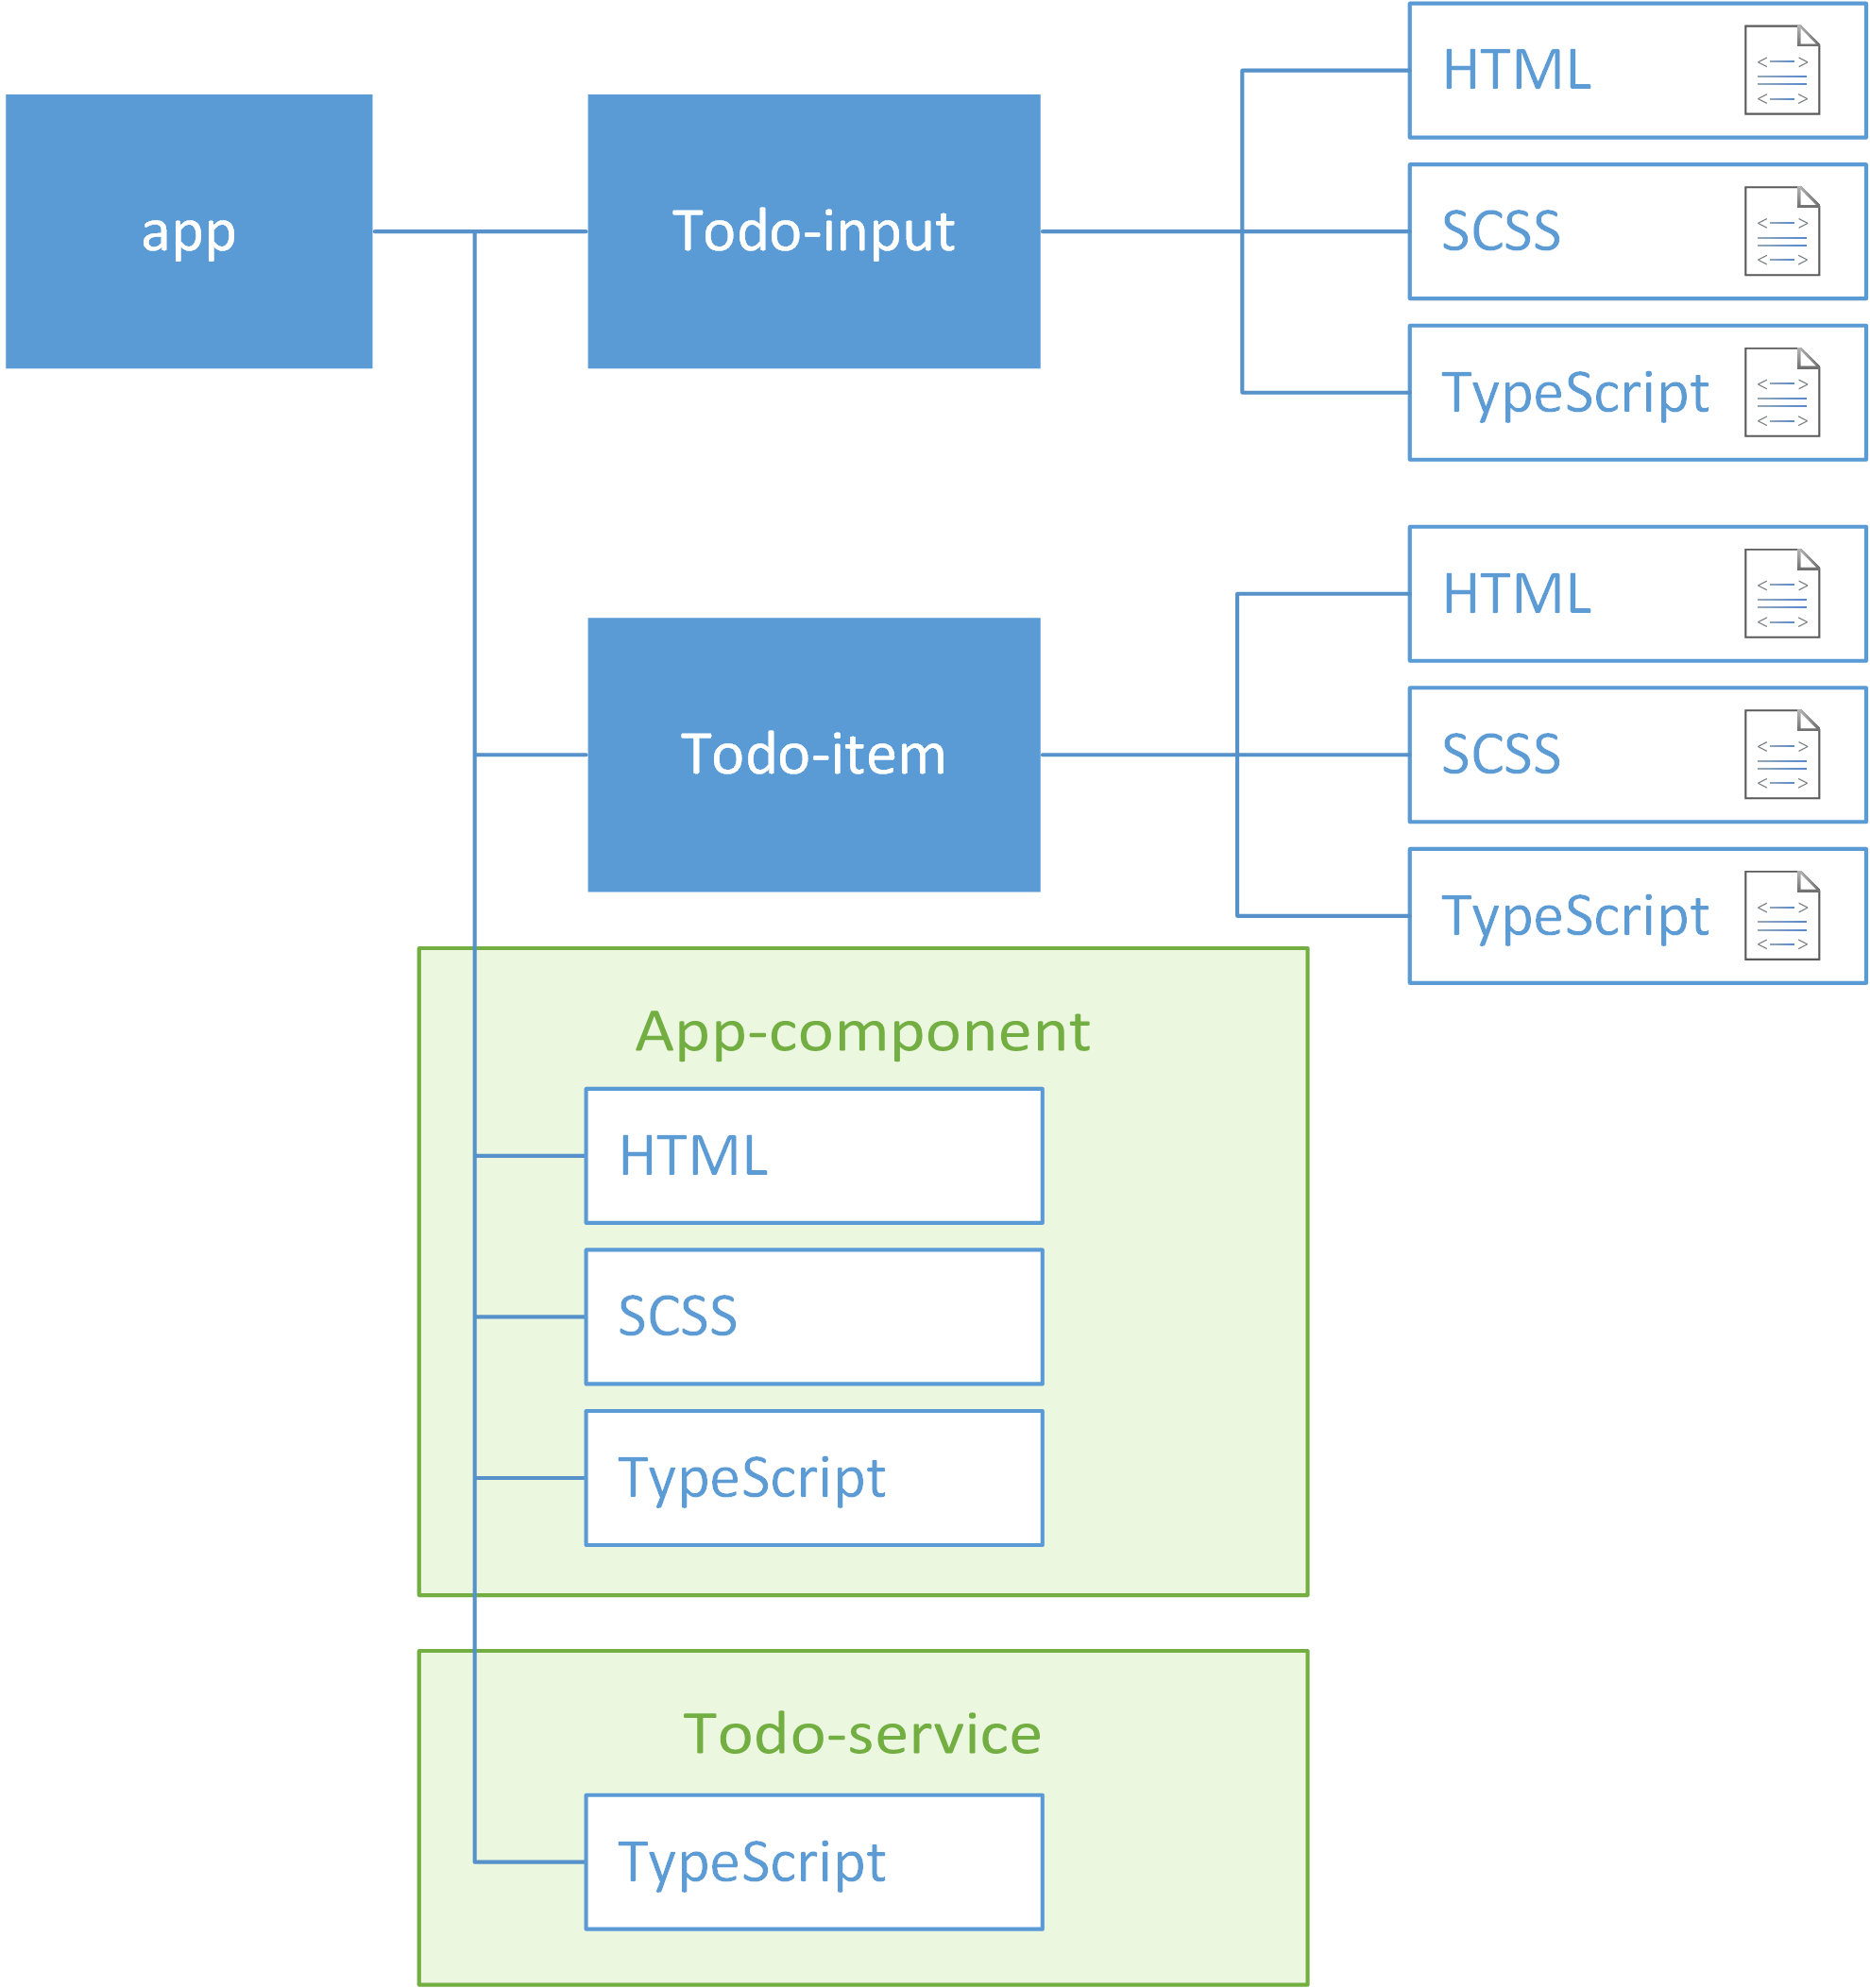
\includegraphics[width=0.6\textwidth]{img/pwa_dateistruktur.png}
	\centering
	\caption{Dateistruktur der Angularanwendung}
	\label{fig:pwa_dateistruktur}
\end{figure}

\begin{description}
	\item[Stammkomponente] Zunächst befinden sich im \texttt{app} Verzeichnis eine HTML-, eine Stylesheet- und eine TypeScript-Datei der \texttt{app-component}: die Stammkomponente. Sie dient als Container (siehe Begrifflichkeiten in Kapitel \ref{chap:grundlagen}) um die Todo-Elemente und das Inputfeld (siehe Ausschnitt \ref{sourcecode:pwa_app_component_html}, Zeile 5).
	

		
	\begin{listing}[h]
		\inputminted{text}{sourcecode/pwa_app_component.html}
		\caption{HTML Template der \texttt{app-component} (gekürzt)}
		\label{sourcecode:pwa_app_component_html}
	\end{listing}

	Ausschnitt \ref{sourcecode:pwa_app_component_html}, Zeilen 1-3, zeigt, wie die Daten aus dem \texttt{todoService} in HTML-Code dargestellt werden. Wie in einer For-Schleife, wird jedes item des \texttt{todoService} einer neu erstellten \texttt{todo-item}-Komponente übergeben.
	Angular wird das HTML-Template automatisch neu rendern, wenn sich die items im \texttt{todoService} ändern.	
	
	
	\item[Todo-item] 
	Das \texttt{todo-item} ist ein einzelnes Elemente der Todo-Liste. Es enthält einen Button zum priorisieren, eine Checkbox zum abhaken des Elements, eine Textbox und einen Button zum Löschen (siehe Abbildung \ref{fig:pwa_todo_item_screenshot}).
	
	\begin{figure}[h]
		
\includegraphics[width=0.6\textwidth]{img/pwa_todo_item.PNG}
		\centering
		\caption{Gerenderte \texttt{todo-item}-Komponente}
		\label{fig:pwa_todo_item_screenshot}
	\end{figure}
	
	
	Es ist sinnvoll jedes Listenelement in einer mehrfach instanziierten Komponente zu repräsentieren. Dies kapselt die Daten des Listenelements und die Kommunikation mit dem \texttt{todoService} von anderen Listenelementen ab. Wie bereits erwähnt bekommt jede \texttt{todo-item}-Komponente genau ein Objekt der Klasse \texttt{TodoItem} übergeben.
	
	\begin{listing}[h]
		\inputminted{text}{sourcecode/pwa_todo_item.html}
		\caption{HTML Template der \texttt{todo-item} (gekürzt)}
		\label{sourcecode:pwa_todo_item_html}
	\end{listing}

	Ausschnitt \ref{sourcecode:pwa_todo_item_html} zeigt das HTML-Template des \texttt{todo-item}. Die ersten drei Input-Elemente werden durch \texttt{[(ngModel)]} mit einer Property des \texttt{TodoItem}s verknüpft, welche in der \texttt{todo-item}-Komponente gespeicht wird. Dies bewirkt folgenden Mechanismus: Wird das Input-Element verändert, ändert sich auch das gespeicherte \texttt{TodoItem}. Würde das \texttt{TodoItem} im Code modifiziert, ändert aktualisiert sich das Input-Element entsprechend.
	
	Um modifizierte Daten auch in der Datenquelle zu speichern, wird das modifizierte \texttt{TodoItem} bei jeder Änderung dem \texttt{todoService} übergeben.
	
	
	
\end{description}

\subsubsection{Kommunikation der Komponenten mit dem \texttt{todoService}}
\begin{figure}[h]
	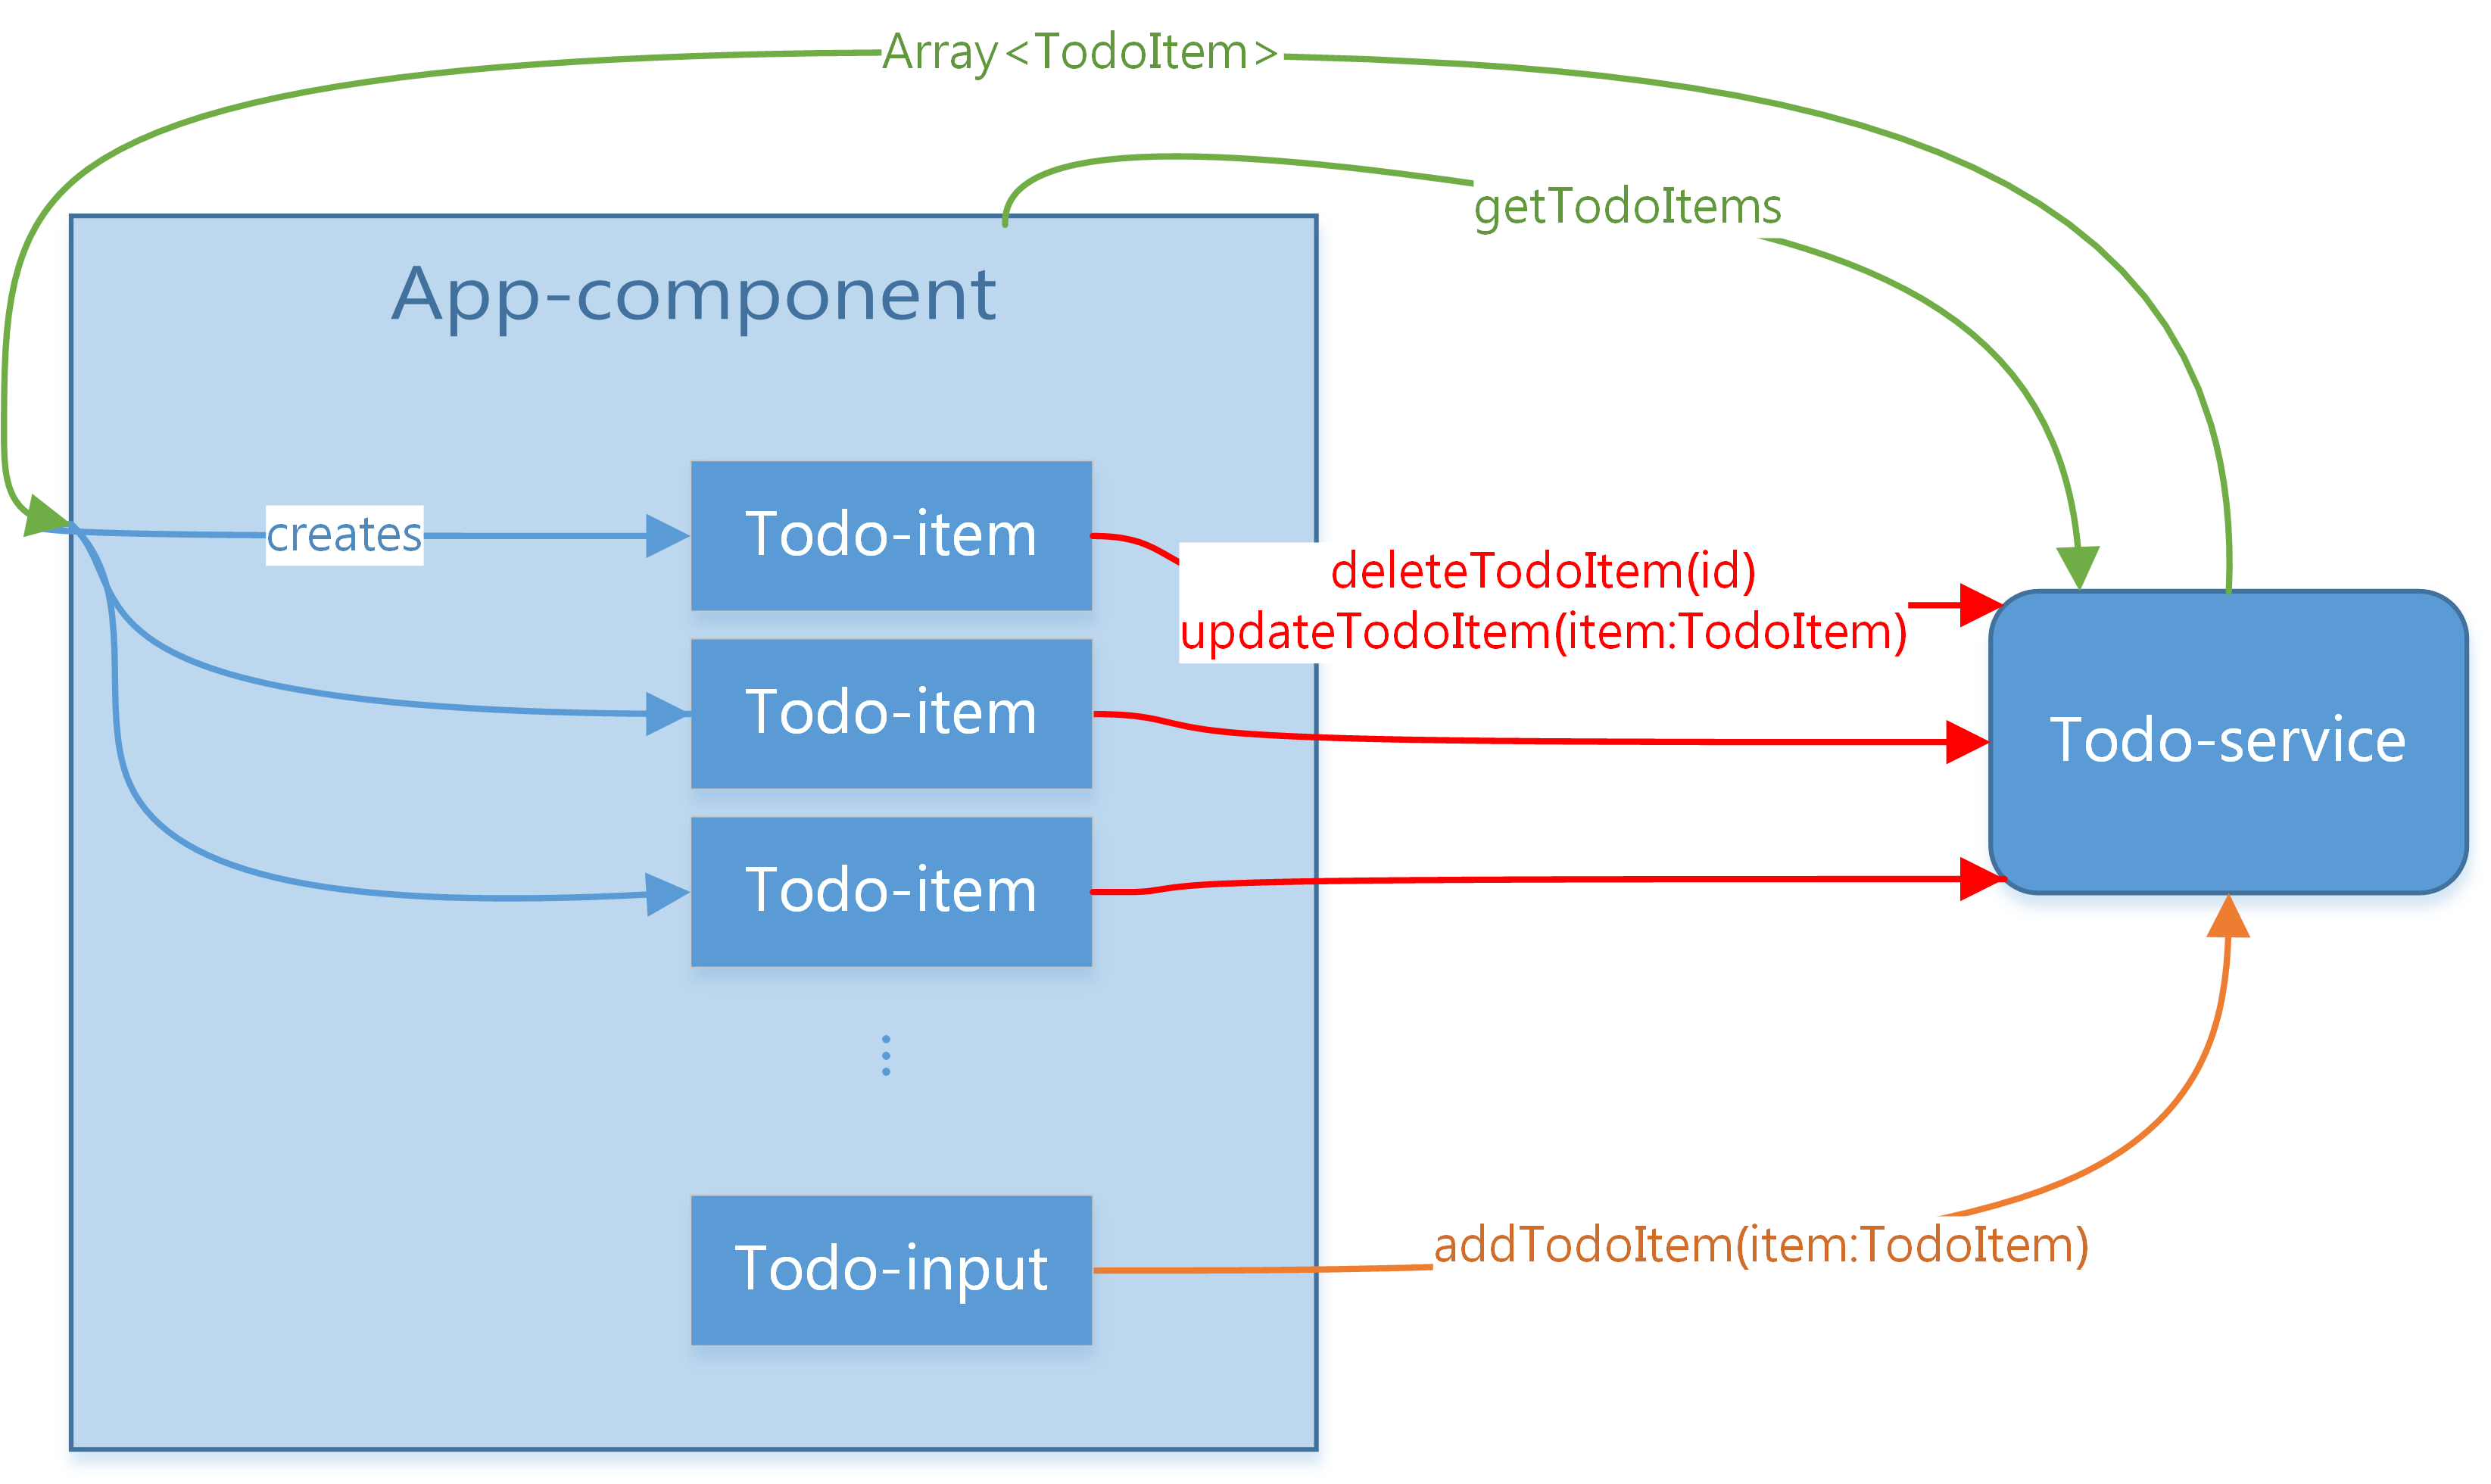
\includegraphics[width=\textwidth]{img/pwa_components.png}
	\centering
	\caption{Interaktion des Todo-service mit den Komponenten}
	\label{fig:pwa_todo_service}
\end{figure}

Abbildung \ref{fig:pwa_todo_service} fasst die Architektur der Angular-Anwendung zusammen. Den zentralen Punkt der Anwendung bildet der \texttt{TodoService}. 

Grün dargestellt ist der Datenfluss der gespeicherten Todo-Elemente zwischen der Stammkomponente und dem \texttt{TodoService}. Die Stammkomponente erhält ein Array aus \texttt{TodoItem}s und wird von Angular automatisch aktualisiert, wenn dieses sich ändert.
Die Stammkomponente erstellt für jedes \texttt{TodoItem} eine \texttt{TodoItem}-Komponente (blau dargestellt), die so als Listeneintrag sichtbar wird.

Orange dargestellt ist das Einfügen von Daten durch den*die Nutzer*in im Inputfeld der App. Der Input stellt dem \texttt{TodoService} ein neues \texttt{TodoItem}-Objekt bereit.

Rot dargestellt ist das Löschen oder Updaten von Items. Wird der Button zum Entfernen gedrückt, oder ändert sich das gespeicherte \texttt{TodoItem}-Objekt der \texttt{TodoItem}-Komponente, werden die Änderungen dem \texttt{TodoService} weitergegeben.
Für das Löschen reicht allerdings die einzigartige ID des Objekts aus.


%\begin{figure}[h]
%	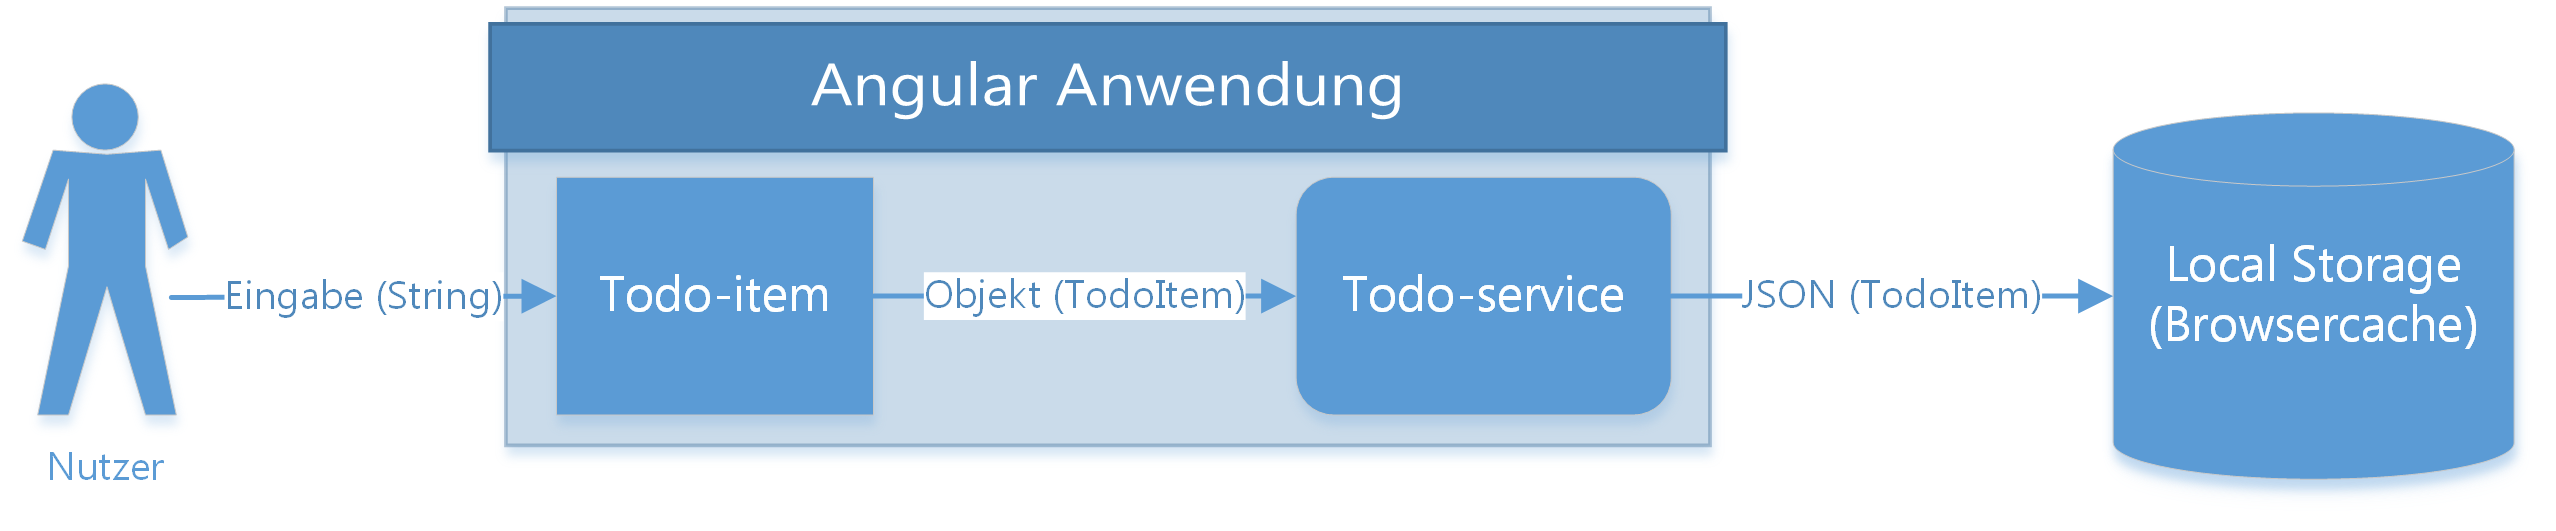
\includegraphics[width=\textwidth]{img/pwa_datenfluss_eingabe.png}
%	\centering
%	\caption{Datenfluss bei Änderung eines Todo Eintrages}
%	\label{fig:pwa_datenfluss_eingabe}
%\end{figure}

\subsection{Integration einer Manifestdatei}

Die Anwendung funktioniert zwar bereits im Browser, ist bislang aber noch keine Progressive Web App. Um dem Projekt ein \textit{Manifest} und einen \textit{Service Worker} hinzuzufügen, kann wieder die Angular \ac{cli} verwendet werden. \texttt{ng add @angular/pwa} erzeugt die entsprechenden Dateien automatisch, fügt eine manifest.json hinzu und bindet diese in die index.html Datei des Projekts ein.

Es ist festzuhalten, dass das hinzufügen der \ac{pwa}-Funktionalität keinen nennenswerten Aufwand mit sich bringt, wenn das Ziel ausschließlich die Installation der Webapp ist.

\subsection{Hosting der App mit Firebase}
Damit die \ac{pwa} als solche installiert werden kann muss sie bestimmte Kriterien erfüllen (siehe Kapitel \ref{chap:grundlagen}). Darunter ist die Notwendigkeit der Bereitstellung über \ac{https}. Dies gestaltet sich in der Praxis als schwierig, da der Angular Entwicklungsserver zwar auf \ac{https} konfiguriert werden kann, jedoch selbstsignierte SSL Zertifikate nicht aktzeptiert werden: Die \ac{pwa} kann nicht installiert werden. Für die Entwicklung ist das natürlich problematisch, so dass eine Lösung für dieses Problem gefunden werden muss.

Für die spätere Evaluierung ist der hier verwendete Hosting-Anbieter nicht relevant. Es gibt zahlreiche Alternativen, die den Anforderungen an das Hosting der Anwendung gerecht werden. Auf diese soll hier aber nicht weiter eingegangen werden. Da das Projekt jedoch aus angeführten Gründen gehostet werden muss, wird das Hosting stellvertretend mit einem Google-Service erläutert.

Googles stellt eine schnelle und elegante Lösung zum Hosten einer Webanwendung bereit: \textit{Firebase}. Über die Firebase Console, eine Webanwendung zur Verwaltung von Firebase Projekten, kann innerhalb weniger Minuten ein Projekt inklusive Hosting erstellt werden. 



Das dem Firebase \ac{cli} können automatisiert Konfigurationsdateien für das Firebase Hosting angelegt werden. Die Schritte dazu sind ebenfalls trivial:
\begin{enumerate}
	\item \textbf{Anmeldung: \\}
	      Das \ac{cli} muss mit einem Google-Konto verknüpft werden. Dazu beim Login über das \ac{cli} ein Browserfenster mit einem Google-Login Dialog.
	\item \textbf{Initialisierung: \\}
	      Die Initialisierung über das \ac{cli} legt unter anderem eine \ac{json}-Datei zur Konfiguration des Deployments an. Hier werden Dateipfade, wie beispielsweise die Start-URL oder Dateien die deployed werden sollen, gespeichert.
	\item \textbf{Deployment: \\}
	      Über die Angular \ac{cli} wird ein sogenannter Production-Build erstellt. Dies ist eine gepackte Version der Webanwendung für den Produktivbetrieb.
	      Anschließend kann die gepackte Anwendung mit \texttt{firebase deploy} auf einem von Googles Servern bereitgestellt werden.
\end{enumerate}

Die Anwendung läuft jetzt mit einer validen \ac{https}-Verbindung und kann von Nutzern installiert werden.

Das Hosting mit Firebase löst gleichzeitig ein weitere Problem: das Testen der Anwendung auf einem Smartphone. Die von Firebase bereitgestellte URL kann jetzt einfach im mobilen Chromebrowser aufgerufen und installiert werden.

\subsection{Installation der Anwendung auf Smartphone und Desktop}
\textbf{Smartphones:}\\
Nach dem Aufrufen der URL mit dem mobilen Browser, erscheint eine Meldung zum Installieren der \ac{pwa} (siehe \ref{fig:dialog_install_pwa_mobile}).

\begin{figure}[h]
	
\includegraphics[scale=0.5]{img/pwa_add_to_homescreen.png}
	\centering
	\caption{Browserdialog zum Installieren der \ac{pwa} als Windows Desktop App}
	\label{fig:dialog_install_pwa_mobile}
\end{figure}

\textbf{Desktop:}
\begin{wrapfigure}{r}{0.5\textwidth}
	\vspace{-10pt}
	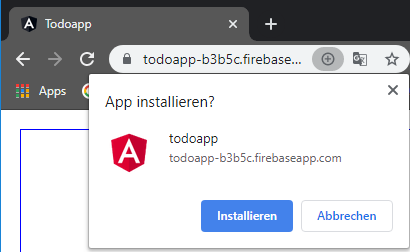
\includegraphics[width=0.48\textwidth]{img/add_to_desktop_2.PNG}
	\caption{Browserdialog zum Installieren der \ac{pwa} als Desktop App}
	\label{fig:dialog_install_pwa_mobile}
	\vspace{-10pt}
\end{wrapfigure}
In der Suchleiste von Chrome, kann der Nutzer die \ac{pwa} als Desktopanwendung installieren (siehe \ref{fig:dialog_install_pwa_mobile}).
\begin{wrapfigure}{L}{0.5\textwidth}
	\vspace{-10pt}
	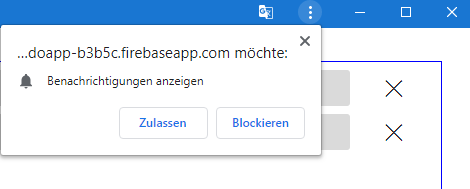
\includegraphics[width=0.48\textwidth]{img/berechtigungen_zulassen.PNG}
	\centering
	\caption{Dialog für Benachrichtigungen}
	\label{fig:pwa_benachrichtigungen_zulassen}
	\vspace{-10pt}
\end{wrapfigure}
Damit dem Nutzer Benachrichtigungen tatsächlich angezeigt werden, muss er beim erhalten der ersten Nachricht die Benachrichtigungen über einen Dialog aktivieren (siehe \ref{fig:pwa_benachrichtigungen_zulassen}).

\subsection{Update der Anwendung}

Um das Updateverhalten zu evaluieren, ist es interessant, den Updateprozess einer Webanwendung beziehungsweise \ac{pwa} zu betrachten. Um Änderungen an die Nutzer zu verteilen, muss ein*e Entwickler*in einen neuen \textit{Production Build} auf dem Server bereitstellen. Im Falle dieses Projekts werden Änderungen unter Nutzung der Firebase \ac{cli} auf den Server übertragen.

In der Praxis werden die Änderungen in der installierte \ac{pwa} nicht sofort sichtbar, wohingegen die Webanwendung beim nächsten Refresh der Seite aktualisiert wird. Dies hängt mit dem Caching der Ressourcen der \ac{pwa} zusammen. Der Service Worker lädt cachbare Dateien entweder beim Start oder nachträglich während die \ac{pwa} läuft in den lokalen Cache des Geräts.

Um dieses Verhalten zu Testen wurde ein Update mit einer auffälligen Hintergrundfarbe auf dem Server bereitgestellt. In der Desktop-\ac{pwa} war die Änderung erst nach einem Systemneustart zu sehen, wohingegen sich die \ac{pwa} unter Android nach einigen Stunden automatisch aktualisiert hatte. Dabei gab es jeweils keine Benachrichtigung zur Aktualisierung für den*die Nutzer*in.






